%!TEX program = xelatex
\documentclass[10pt, compress]{beamer}

\usetheme{m}

\usepackage{booktabs}
\usepackage[scale=2]{ccicons}
\usepackage{minted}

\usemintedstyle{trac}

\title{Reconhecimento da Fala a Partir de Espectrograma usando MobileNetV2}
\subtitle{Projeto Demonstrativo 6 - Visão Computacional}
\date{\today}
\author{Igor Bispo  \and igor.rabbit99@gmail.com \\ Hevelyn Sthefany \and hevelyn.sthefany@gmail.com}

\institute{
  Departamento de Ciência da Comptutação\\
  Universidade de Brasília\\
  Campus Darcy Ribeiro, Asa Norte\\
  Brasília-DF, CEP 70910-900, Brazil,}

\begin{document}

\maketitle

\begin{frame}[fragile]
  \frametitle{Sumário}
  \tableofcontents
\end{frame}




\section{Reconhecimento da Fala} %-----------------------------------------------------------

\begin{frame}[fragile]
  \frametitle{Reconhecimento da Fala}
  \begin{center}O reconhecimento de fala é uma tecnologia que procura identificar palavras faladas em um áudio e convertê-las em texto.\end{center}

  \begin{figure}
  \centering
  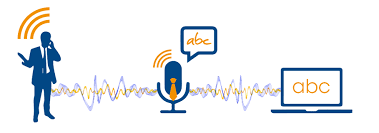
\includegraphics[scale=0.5]{images/speechrec.png}
    %\caption{Rotated square from
    %\href{http://www.texample.net/tikz/examples/rotated-polygons/}{texample.net}.}
  \end{figure}
\end{frame}


\begin{frame}
  \alert{Siri}, \alert{Open Mic+}, \alert{Siri}, \alert{Siri} são exemplos de aplicações que usam reconhecimento da fala.
\end{frame}


\begin{frame}{Reconhecimento com Espectrograma usando MobileNetV2}
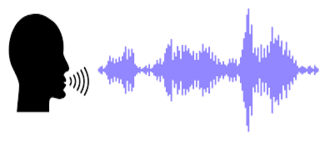
\includegraphics[scale=0.35]{images/process-11.png}
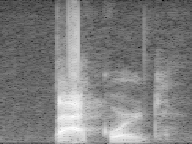
\includegraphics[scale=0.15]{images/process-2.png}
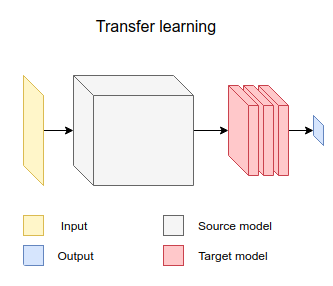
\includegraphics[scale=0.3]{images/process-3.png}

\includegraphics[scale=0.01]{images/process-4.jpg}
\end{frame}


\section{Espectrograma} %---------------------------------------------------------------------
\begin{frame}{Espectrograma}
\centering
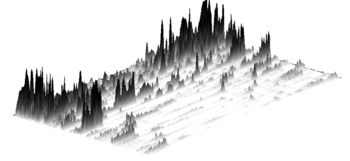
\includegraphics[scale=0.4]{images/spect1.png}
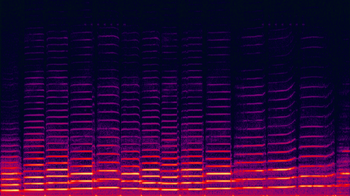
\includegraphics[scale=0.4]{images/spect2.png}
\\
\begin{center} Gráficos que analisam dinamicamente a densidade espectral de energia. Os valores são indicados no plano \alert{tempo} X \alert{frequência} e cores indicam \alert{intensidade} da densidade espectral de energia. \end{center}
\end{frame}

\begin{frame}
\centering
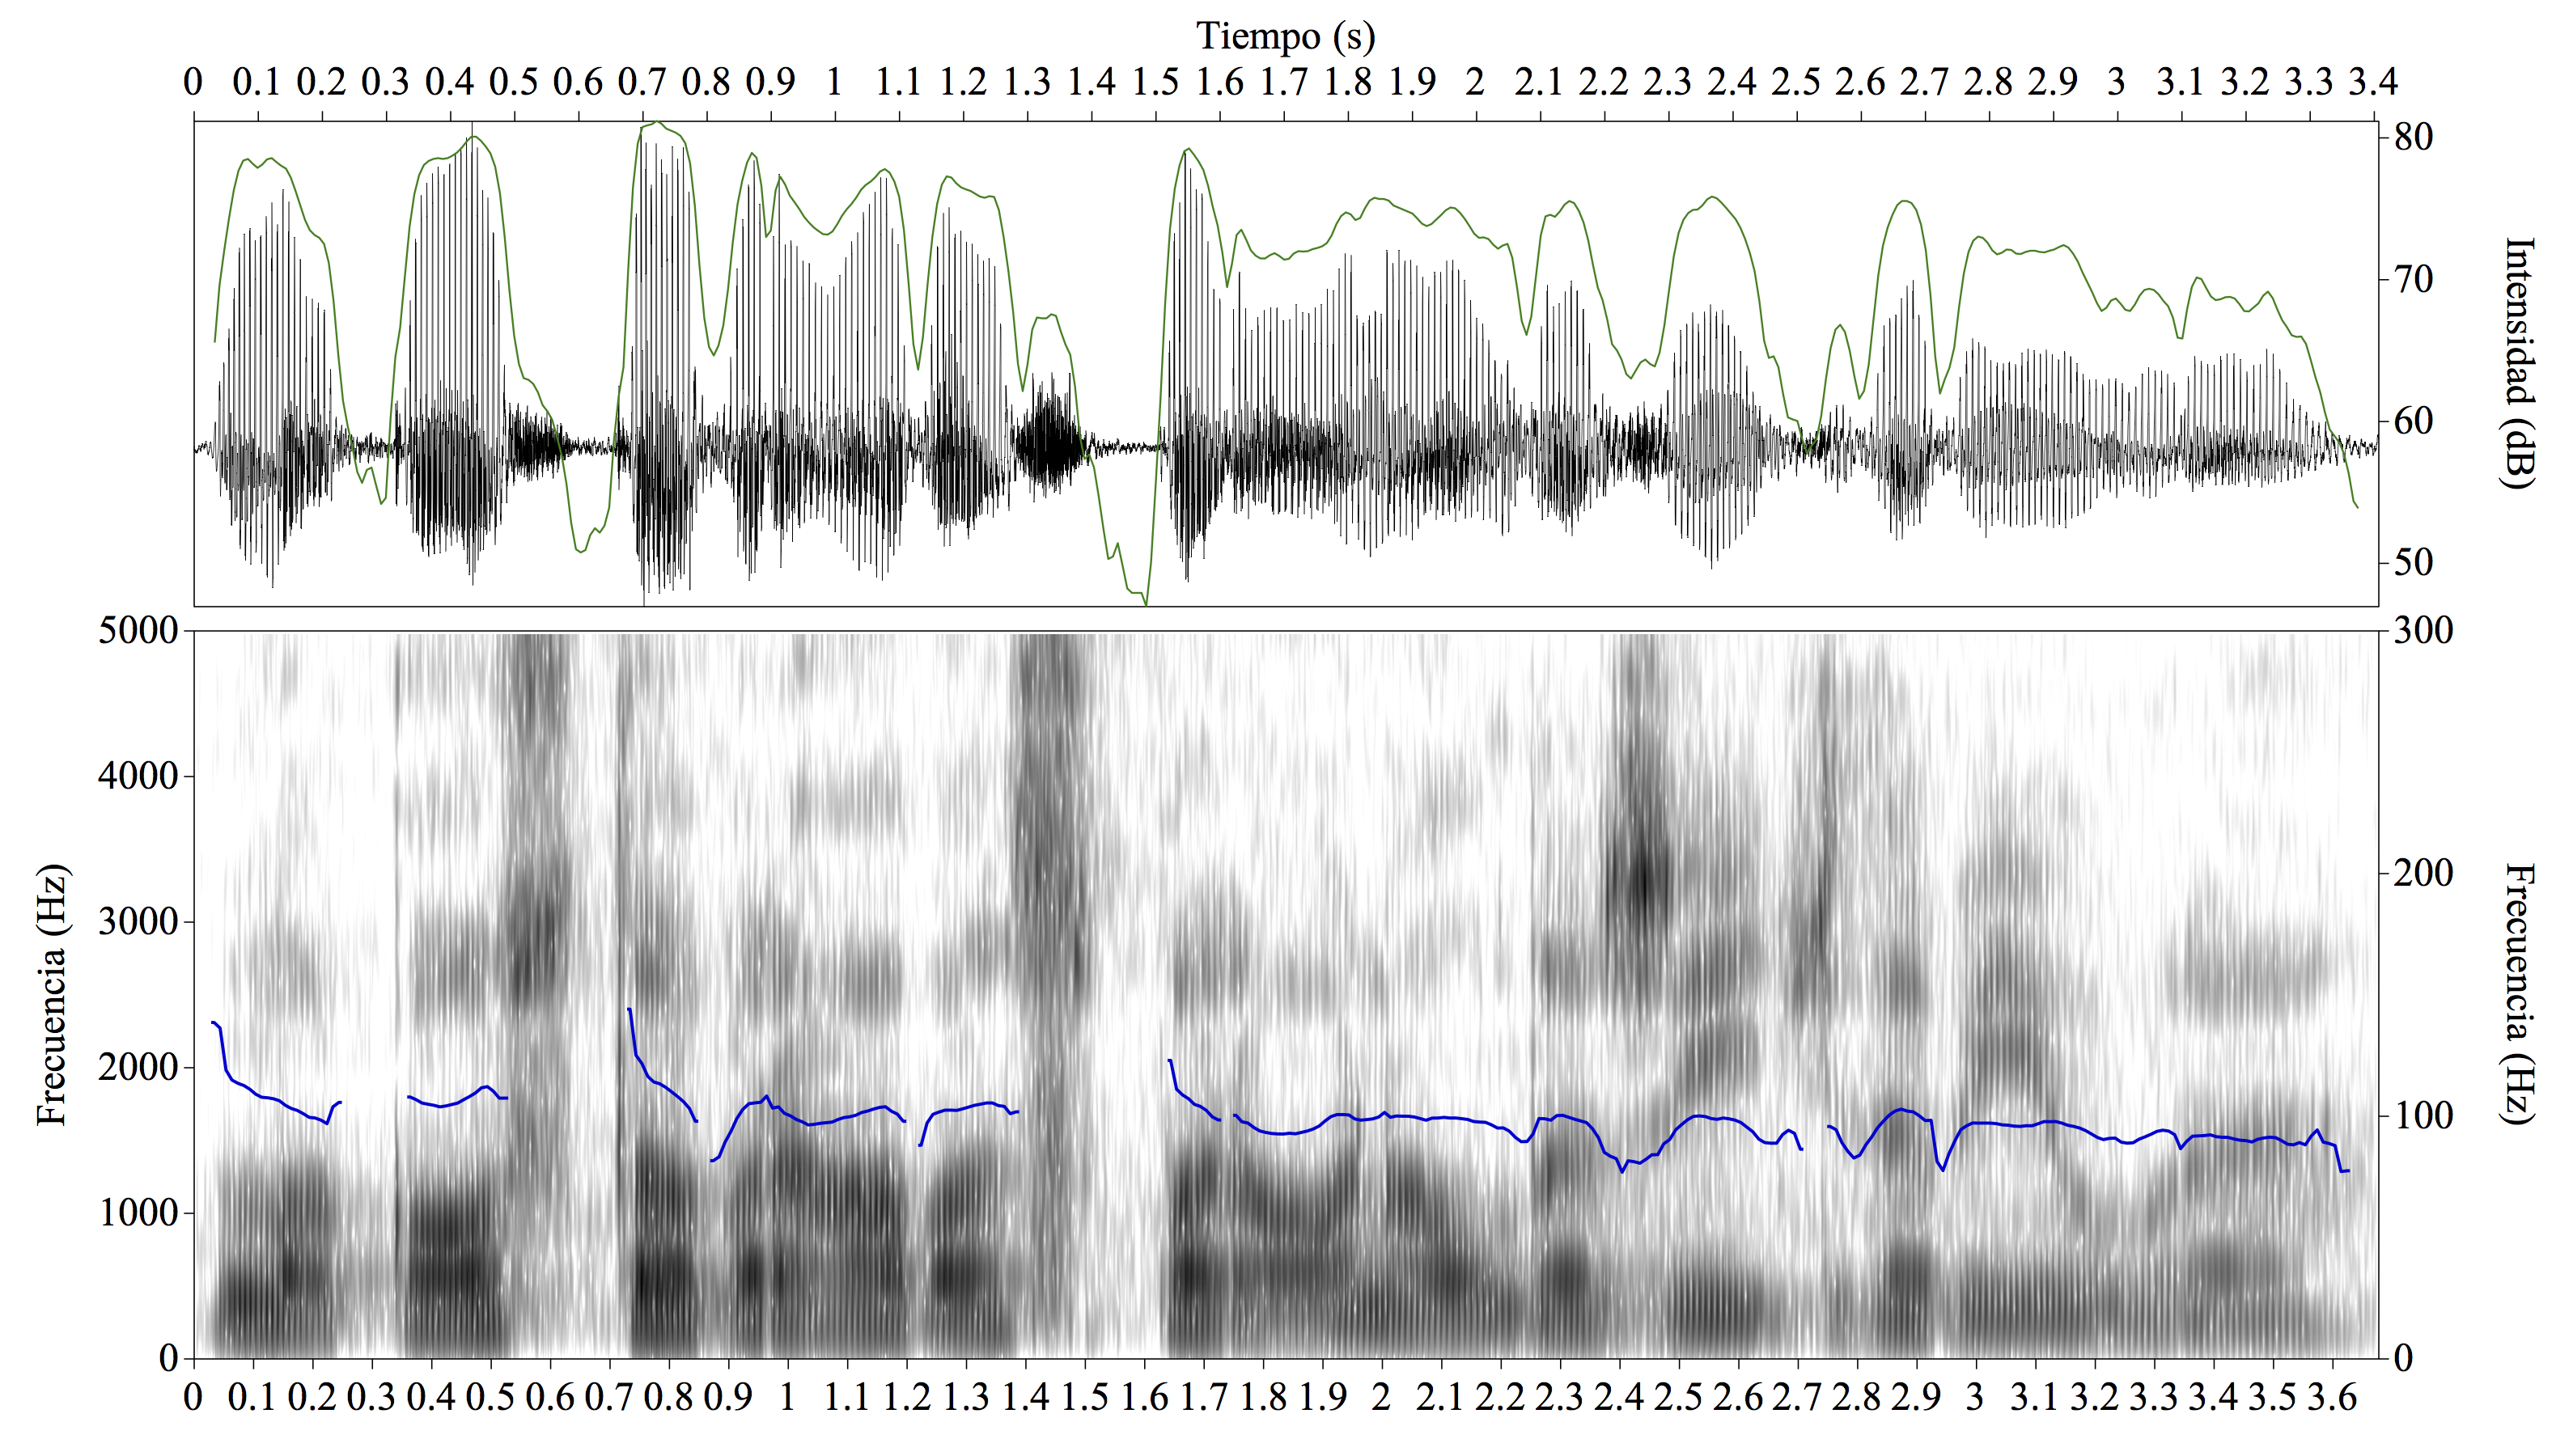
\includegraphics[scale=0.1]{images/spect3.jpg}
\end{frame}

\section{MobileNetV2} %---------------------------------------------------------------------
\begin{frame}{MobileNetV2}
  \begin{description}
    \centering
    \item[Convoluções Separáveis em Profundidade] Além de mapear uma única convolução em cada canal de entrada separadamente, adiciona a etapa da  Convolução Pontual: Convolução com um tamanho de kernel de 1x1 que combina os recursos criados pela convolução em profundidade.

    \item[Resíduos Invertidos] Blocos residuais conectam o início e o fim de um bloco convolucional com uma conexão de salto.

    \item[Gargalos] Última convolução de um bloco residual tem uma saída linear antes de ser adicionada às ativações iniciais.
  \end{description}
\end{frame}


\begin{frame}{Convoluções Separáveis}
\begin{figure}
\centering
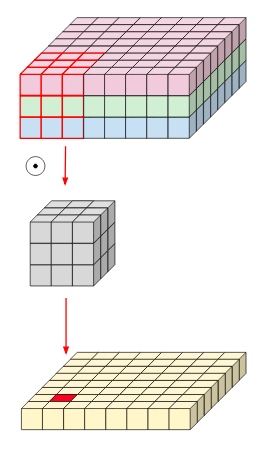
\includegraphics[scale=0.25]{images/conv1.png} \hfil
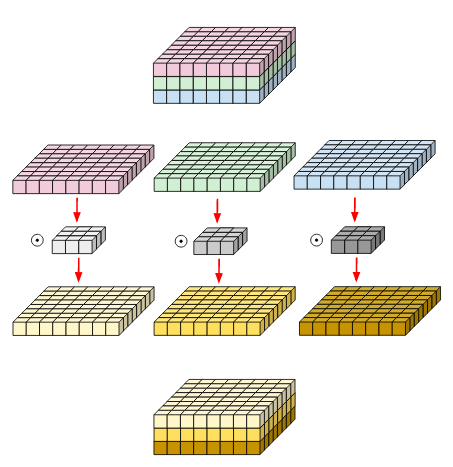
\includegraphics[scale=0.25]{images/conv2.png} \hfil
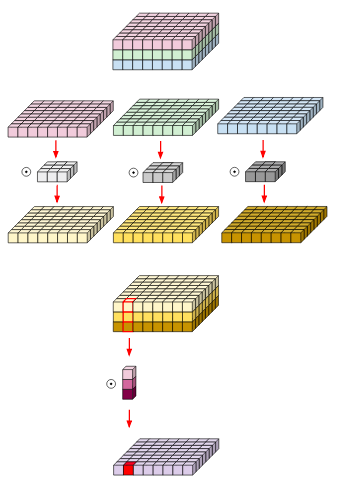
\includegraphics[scale=0.25]{images/conv3.png}
\caption{Na sequência: Convolução Normal, Convolução Profunda e Convolução Separável Profunda}
\end{figure}
\end{frame}

\begin{frame}{Resíduos Invertidos}
\begin{figure}
\centering
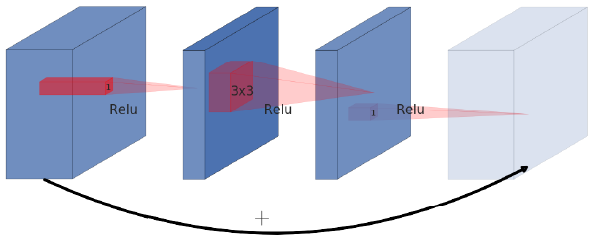
\includegraphics[scale=0.25]{images/noinvert.png}
\caption{Um bloco residual conecta camadas largas com uma conexão de salto, enquanto as camadas intermediárias são estreitas}
\end{figure}

\begin{figure}
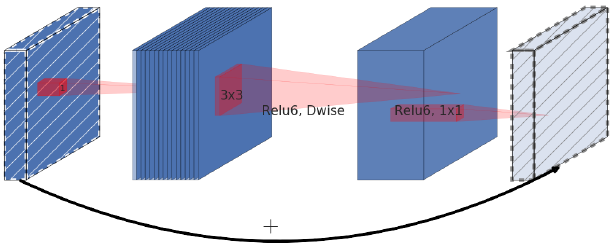
\includegraphics[scale=0.25]{images/invert.png}
\caption{Um bloco residual invertido conecta camadas estreitas com uma conexão de salto enquanto as camadas intermediárias são largas}
\end{figure}
\end{frame}


\begin{frame}{Gargalos Lineares}

A última convolução de um bloco residual tem uma \alert{saída linear} antes de ser adicionada às ativações iniciais. Colocar isso no código é super simples, pois simplesmente descartamos a última função de ativação do bloco convolucional.
\end{frame}

\section{Resultados} %---------------------------------------------------------------------------

\begin{frame}{Espectrograma ``right''}
\centering
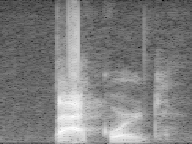
\includegraphics[scale=0.5]{images/process-2.png}\\
Espectrograma classificado corretamente como "right" com \alert{99\%} de confiança.
\end{frame}

\begin{frame}{Filtro aplicado na Convolução para espectrograma}
\begin{figure}
\centering

\includegraphics[scale=6]{images/filtrospeech.png} 
\end{figure}
\end{frame}

\begin{frame}{Filtro aplicado na Convolução para reconhecimento de objetos}
\begin{figure}
\centering
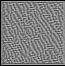
\includegraphics[scale=8]{images/filtroobj.png}
\end{figure}
\end{frame}


\begin{frame}{Relatório de Classificação}
\begin{table}[htbp]
\centering
\begin{tabular}{|c|c|c|c|c|}
\hline
             & precision  &  recall & f1-score &  support \\ \hline

         bed &      0.95  &    0.98  &    0.97 &      500 \\ \hline
        bird &      0.96  &    0.99  &    0.98 &      500 \\ \hline
         cat &      0.96  &    0.99  &    0.97 &      500 \\ \hline
         dog &      0.97  &    0.96  &    0.97 &      500 \\ \hline
        down &      0.95  &    0.93  &    0.94 &      500 \\ \hline
       eight &      0.95  &    0.97  &    0.96 &      500 \\ \hline
        five &      0.98  &    0.91  &    0.94 &      500 \\ \hline
        four &      0.97  &    0.93  &    0.95 &      500 \\ \hline
          go &      0.88  &    0.95  &    0.92 &      500 \\ \hline
       happy &      1.00  &    0.99  &    0.99 &      500 \\ \hline
       house &      0.99  &    0.99  &    0.99 &      500 \\ \hline
        left &      0.99  &    0.95  &    0.97 &      500 \\ \hline
      marvin &      0.99  &    0.98  &    0.99 &      500 \\ \hline
        nine &      0.96  &    0.95  &    0.96 &      500 \\ \hline
          no &      0.99  &    0.86  &    0.92 &      500 \\ \hline
\end{tabular}
\end{table}
\end{frame}

\begin{frame}{Relatório de Classificação}
\begin{table}
\begin{tabular}{|c|c|c|c|c|}
\hline
         off &      0.98  &    0.93  &    0.96 &      500 \\ \hline
          on &      0.95  &    0.94  &    0.95 &      500 \\ \hline
         one &      0.97  &    0.94  &    0.96 &      500 \\ \hline
       right &      0.99  &    0.95  &    0.97 &      500 \\ \hline
       seven &      0.95  &    0.98  &    0.96 &      500 \\ \hline
      sheila &      0.99  &    0.98  &    0.98 &      500 \\ \hline
         six &      0.94  &    0.98  &    0.96 &      500 \\ \hline
        stop &      0.94  &    0.95  &    0.94 &      500 \\ \hline
       three &      0.99  &    0.97  &    0.98 &      500 \\ \hline
         two &      0.97  &    0.96  &    0.96 &      500 \\ \hline
          up &      0.95  &    0.96  &    0.95 &      500 \\ \hline
         wow &      0.98  &    0.98  &    0.98 &      500 \\ \hline
         yes &      0.98  &    0.98  &    0.98 &      500 \\ \hline
        zero &      0.97  &    0.95  &    0.96 &      500 \\ \hline

   micro avg &      \alert{0.97}   &   0.92  &    0.96 &    14500 \\ 
weighted avg &      0.97   &   0.96  &    0.96 &    14500 \\ \hline
\end{tabular}
\end{table}
\end{frame}

\begin{frame}{Matriz de Confusão - 10 epochs}
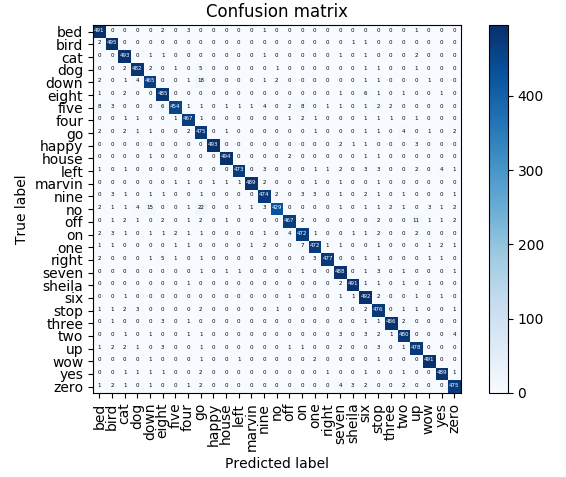
\includegraphics[scale=0.5]{images/mtxc.png}
\end{frame}


%\plain{Dark background}{\vspace{-2em}\begin{center}\includegraphics[width=\textwidth]{images/valley.jpg}\end{center}}

\section{Conclusão}

\plain{}{Obrigado!}

\end{document}
